\documentclass[12pt, a4paper]{article}
\usepackage[a4paper, margin=2.5cm]{geometry}
\usepackage[utf8]{inputenc}
\usepackage[swedish]{babel}
\usepackage{amsmath}
\usepackage{siunitx}

\usepackage{graphicx}
\graphicspath{ {images/} }

\usepackage{parskip}
\usepackage{dirtytalk}

\usepackage{fancyhdr}
\pagestyle{fancy}
\fancyhead[L]{\textbf{Namn:} Björn Sundin}
\fancyhead[C]{\textbf{Klass:} TE18C}
\fancyhead[R]{\textbf{Skola:} NTI Kronhus}

\title{Labbrapport: dämpad och driven pendel}
\author{Björn Sundin\medskip\\ TE18C, NTI Kronhus}

\begin{document}

\maketitle

\section{Inledning}
\subsection{Syfte}
I denna laboration undersöks en torsionspendel. Syftet är att ta reda på egenskaper hos pendeln från data som samlas från sensorer vid svängningar med olika dämpnings\-koefficient samt med och utan ett pålagt periodiskt vridmoment med varierande frekvens.
\subsection{Frågeställningar}
\begin{enumerate}
    \item Vad är torsionspendelns egenfrekvens?
    \item Vad är frekvensen hos drivningsenheten som ger resonans i pendeln?
    \item Vad är förhållandet mellan dämpningskonstanten $\lambda$ och spänningen $U$ på dämp\-ningsenheten?
    \item Hur väl beskriver de matematiska modellerna systemet?
\end{enumerate}

\subsection{Teori}
Den matematiska modellen som används för att beskriva svängningsrörelsen hos torsionspendeln beskrivs av denna differentialekvation:
\begin{equation}
    \begin{split}
        I\frac{\mathrm{d}^2\theta}{\mathrm{d}t^2}=-k\theta-\lambda\frac{\mathrm{d}\theta}{\mathrm{d}t}+\mu\cos(\omega t)\Leftrightarrow\\
        \theta''(t)+\frac{\lambda}{I}\theta'(t)+\frac{k}{I}\theta(t)=\frac{\mu}{I}\cos(\omega t)
    \end{split}
\end{equation}
Där: 
\begin{itemize}
    \item $\theta$ är vinkelpositionen av pendeln relativt jämviktsläget i radianer.
    \item $I$ är tröghetsmomentet för pendeln med enhet \si{kg.m^2}. Det är vridmomentet som krävs för att skapa en vinkelacceleration på 1 \si{rad/s^2}.
    \item $k$ är vridmomentet per radian vinkelavvikelse riktat mot jämviktsläget för den specifika pendeln. Detta vridmoment orsakar den naturliga svängningen.
    \item $\lambda$ är ett bromsande vridmoment per \si{rad/s} motriktat rörelseriktningen. Denna orsakar pendelns dämpning.
    \item $\mu$ är amplituden av det pålagda vridmomentet, med frekvensen $\omega$ \si{rad/s}.
\end{itemize}
$I$, $k$ och $\lambda$ beror alla på egenskaper hos pendeln samt pendelns radie. $\mu$ beror däremot på den radie där det pålagda vridmomentet appliceras samt kraftens maximum som orsakar vridmomentet.

Differentialekvationen har olika lösningar beroende på värdena på konstanterna:
\begin{enumerate}
    \item Fri pendel, $\mu=0\land\lambda=0$
    \begin{equation}\label{eq:fri_pendel}
        \theta(t)=A\sin\biggl(t\sqrt\frac{k}{I}+\phi\biggr)
    \end{equation}
    \item Svagt dämpad pendel, $\mu=0\land\lambda<2\sqrt{Ik}$
    \begin{equation}\label{eq:svagt_dämpad}
        \theta(t)=Ae^{-\frac{\lambda}{2I}t}\sin\biggl(t\sqrt{\frac{k}{I}-\frac{\lambda^2}{4I^2}}+\phi\biggr)
    \end{equation}
    \item Kritiskt dämpad pendel, $\mu=0\land\lambda=2\sqrt{Ik}$
    \begin{equation}
        \theta(t)=e^{-\frac{\lambda}{2I}t}\left(C_1t+C_2\right)
    \end{equation}
    \item Starkt dämpad pendel, $\mu=0\land\lambda>2\sqrt{Ik}$
    \begin{equation}\label{eq:starkt_dämpad}
        \theta(t)=e^{-\frac{\lambda}{2I}t}\left(C_1e^{t\sqrt{\frac{\lambda^2}{4I^2}-\frac{k}{I}}}+C_2e^{-t\sqrt{\frac{\lambda^2}{4I^2}-\frac{k}{I}}}\right)
    \end{equation}
    \item Driven pendel, $\mu\neq0\land\lambda=0$
    \begin{equation}
        \theta(t)=\frac{\mu}{\omega_0^2-\omega^2}\sin\left(\omega t+\phi\right)
    \end{equation}
    Där $\omega$ är den drivande frekvensen och $\omega_0$ är egenfrekvensen.
\end{enumerate}
\section{Metod}

\section{Resultat}
Den insamlade datan som mättes med Cassy Lab under laborationen redovisas i figurerna nedan. 

\begin{figure}[hp]
    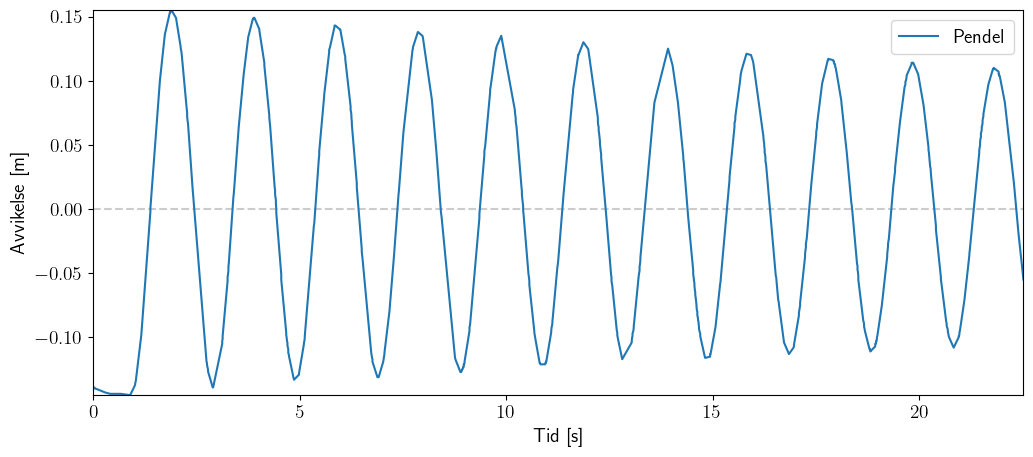
\includegraphics[width=\textwidth]{graf_egenfrekvens}
    \caption{Datan för svängning utan pålagd dämpning.}
    \label{fig:data_egenfrekvens}
\end{figure}

\begin{figure}[hp]
    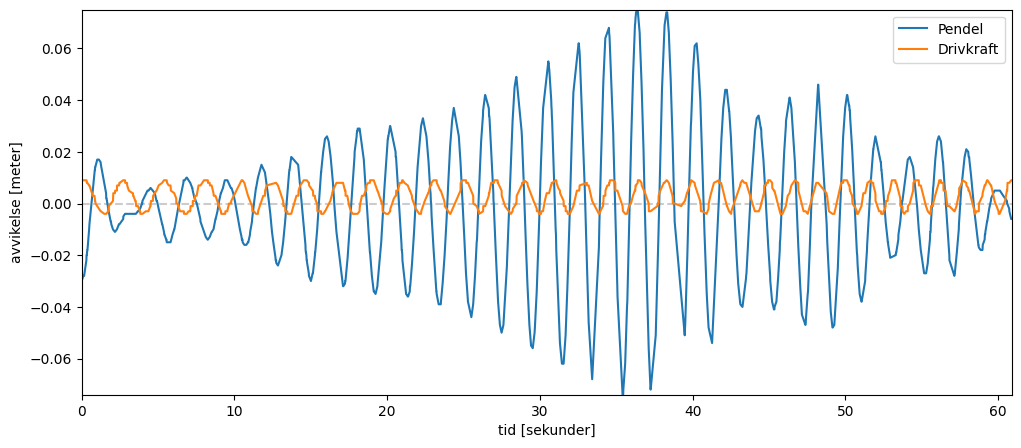
\includegraphics[width=\textwidth]{graf_resonansfrekvens}
    \caption{Datan för driven svängning runt resonansfrekvensen.}
    \label{fig:data_resonansfrekvens}
\end{figure}

\begin{figure}[hp]
    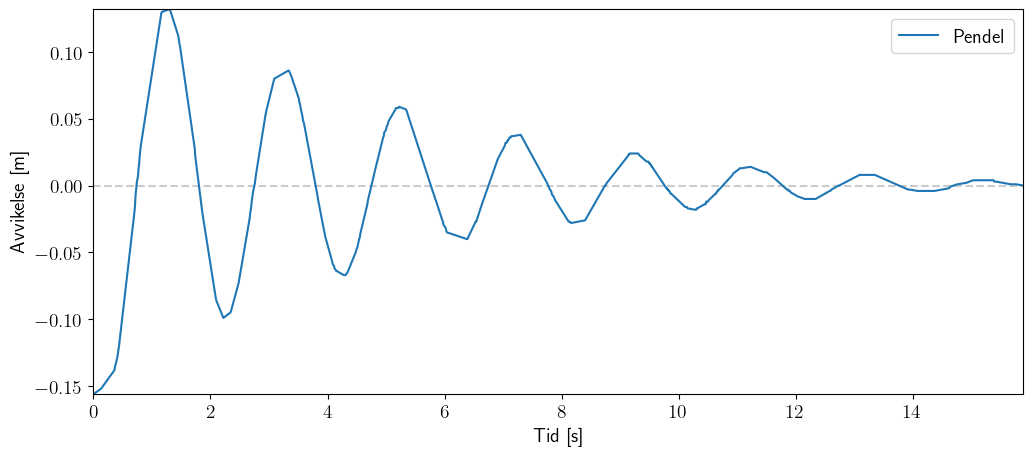
\includegraphics[width=\textwidth]{graf_1_v_centered}
    \caption{Datan för dämpad svängning med 1 V spänning i dämpningsenheten.}
    \label{fig:data_1_v}
\end{figure}

\begin{figure}[hp]
    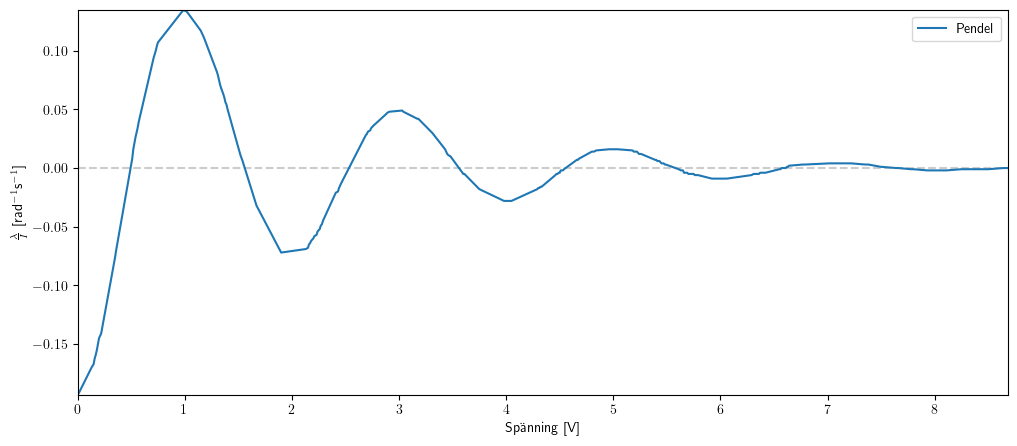
\includegraphics[width=\textwidth]{graf_4_v_centered}
    \caption{Datan för dämpad svängning med 4 V spänning i dämpningsenheten.}
    \label{fig:data_4_v}
\end{figure}

\begin{figure}[hp]
    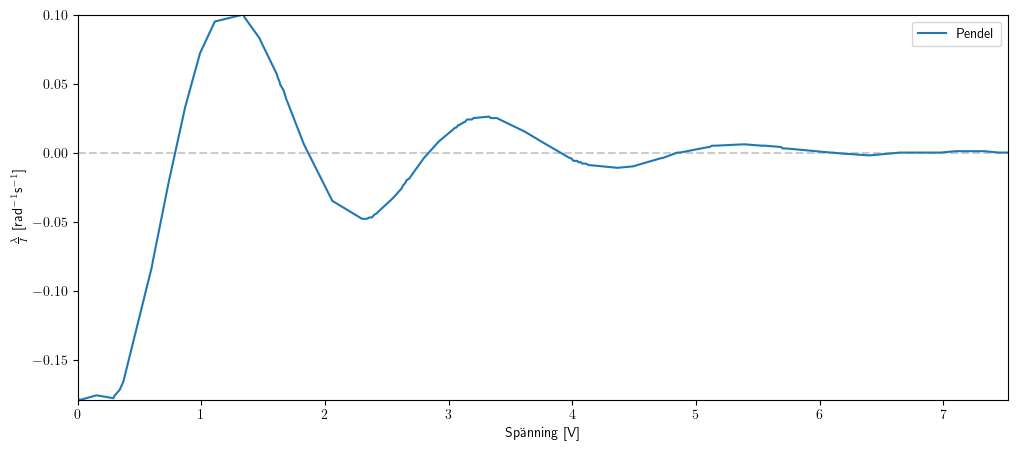
\includegraphics[width=\textwidth]{graf_5_v_centered}
    \caption{Datan för dämpad svängning med 5 V spänning i dämpningsenheten.}
    \label{fig:data_5_v}
\end{figure}

\begin{figure}[hp]
    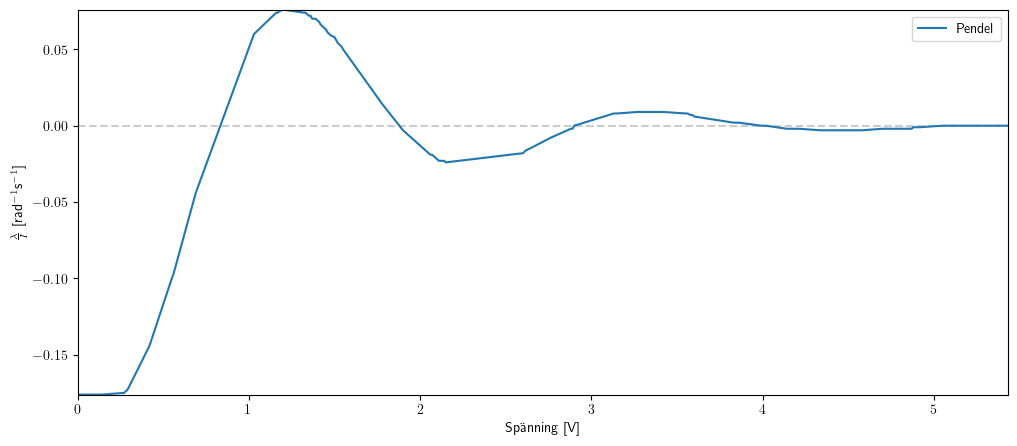
\includegraphics[width=\textwidth]{graf_6_v_centered}
    \caption{Datan för dämpad svängning med 6 V spänning i dämpningsenheten.}
    \label{fig:data_6_v}
\end{figure}

\begin{figure}[hp]
    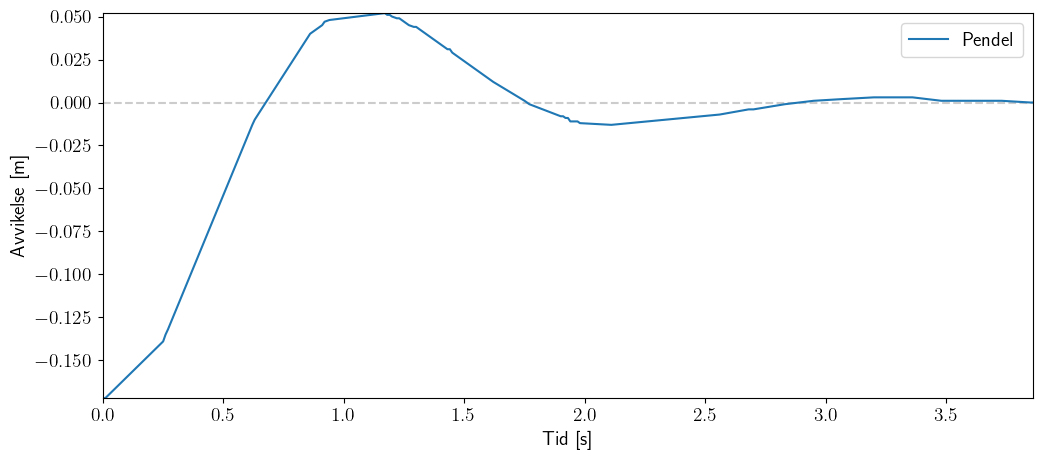
\includegraphics[width=\textwidth]{graf_7_v_centered}
    \caption{Datan för dämpad svängning med 7 V spänning i dämpningsenheten.}
    \label{fig:data_7_v}
\end{figure}

\begin{figure}[hp]
    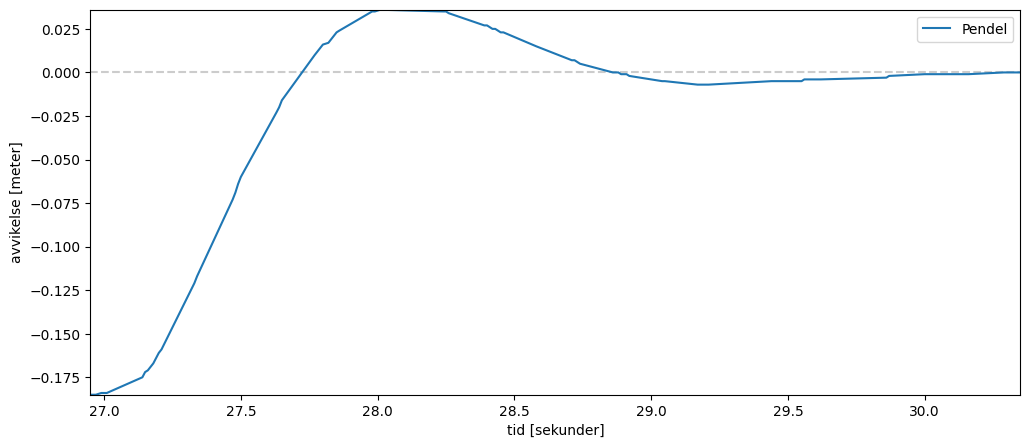
\includegraphics[width=\textwidth]{graf_8_v_centered}
    \caption{Datan för dämpad svängning med 8 V spänning i dämpningsenheten.}
    \label{fig:data_8_v}
\end{figure}

\begin{figure}[hp]
    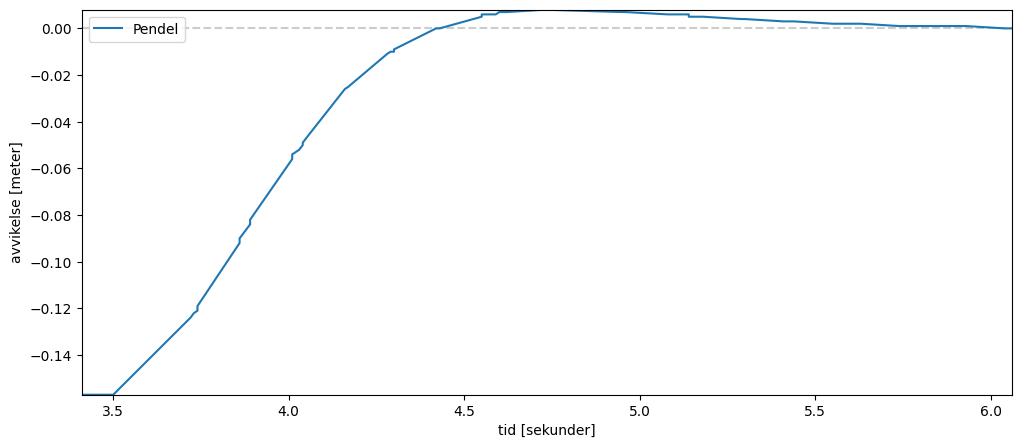
\includegraphics[width=\textwidth]{graf_9_v_centered}
    \caption{Datan för dämpad svängning med 9 V spänning i dämpningsenheten.}
    \label{fig:data_9_v}
\end{figure}

\begin{figure}[hp]
    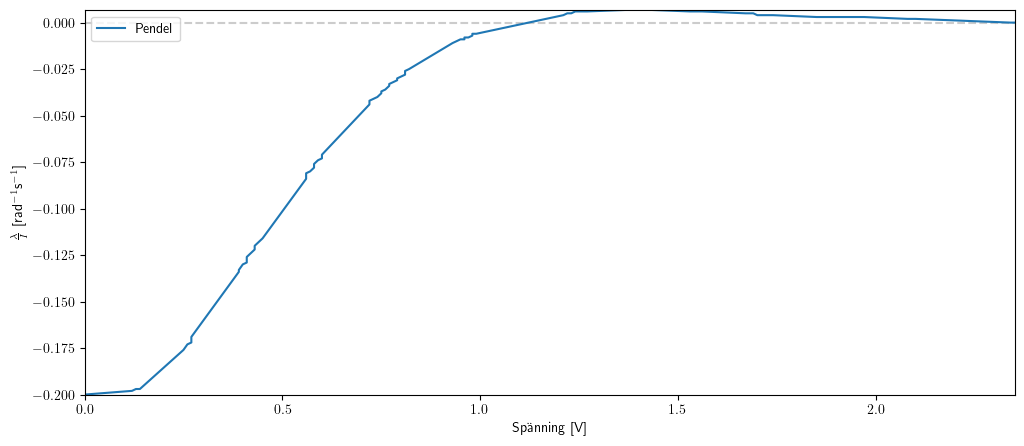
\includegraphics[width=\textwidth]{graf_10_v_centered}
    \caption{Datan för dämpad svängning med 10 V spänning i dämpningsenheten.}
    \label{fig:data_10_v}
\end{figure}

\begin{figure}[hp]
    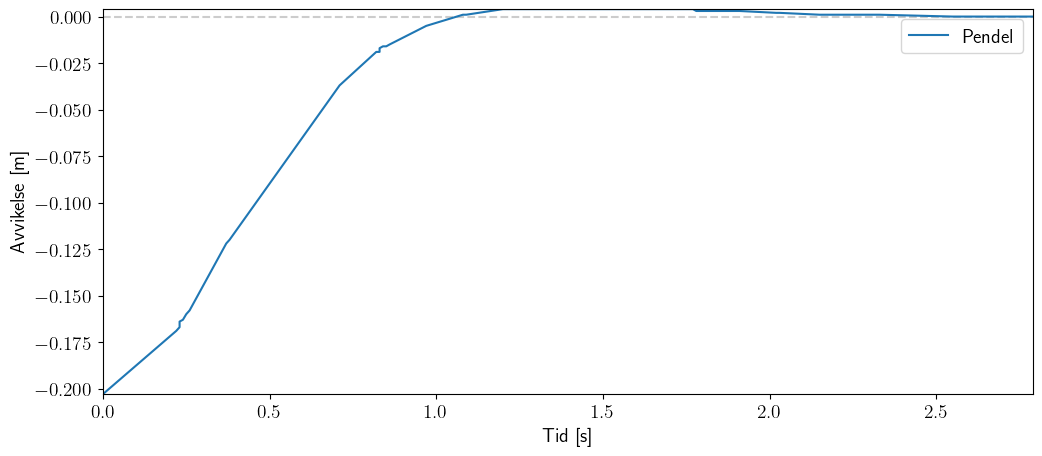
\includegraphics[width=\textwidth]{graf_11_v_centered}
    \caption{Datan för dämpad svängning med 11 V spänning i dämpningsenheten.}
    \label{fig:data_11_v}
\end{figure}

\begin{figure}[hp]
    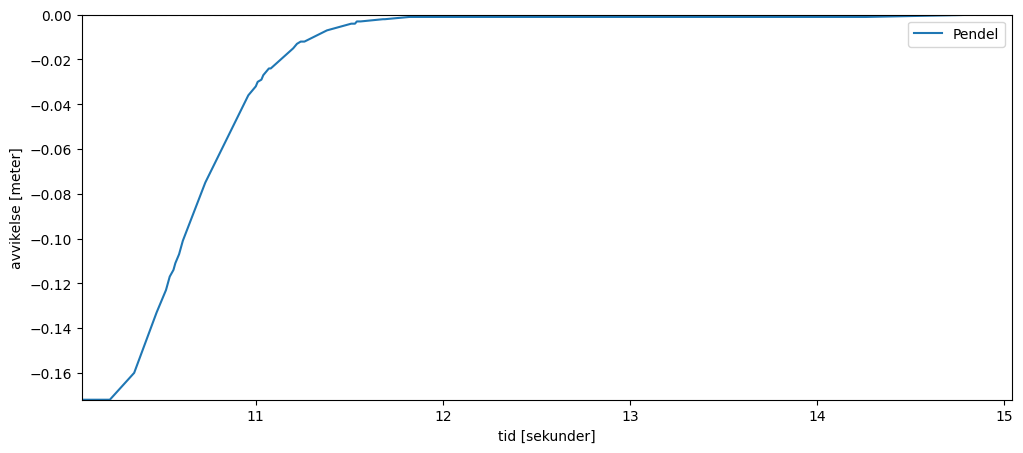
\includegraphics[width=\textwidth]{graf_13_v_centered}
    \caption{Datan för dämpad svängning med 13 V spänning i dämpningsenheten.}
    \label{fig:data_13_v}
\end{figure}

\begin{figure}[hp]
    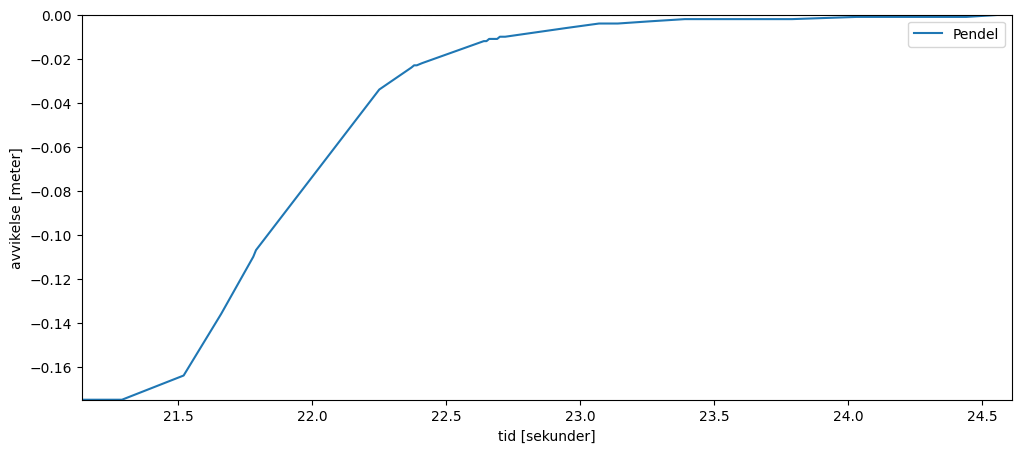
\includegraphics[width=\textwidth]{graf_14_v_centered}
    \caption{Datan för dämpad svängning med 14 V spänning i dämpningsenheten.}
    \label{fig:data_14_v}
\end{figure}

\clearpage
\section{Analys}

En funktionsanpassning av datan i Figur \ref{fig:data_egenfrekvens} med lösningen i ekvation \ref{eq:fri_pendel} gav:
\begin{equation}
    \theta(t)=0.125665\cdot\sin\bigl(3.15192t+1.81944\bigr)
\end{equation}
% En funktionsanpassning av samma data med ekvation \ref{eq:}

Egenfrekvensen är alltså $\omega_0=\sqrt\frac{k}{I}=\SI{3.15192}{rad/s}$, amplituden $A=\SI{0.125665}{m}$, och fas\-förskjutningen $\phi=\SI{1.81944}{rad}$.

\begin{figure}[hp]
    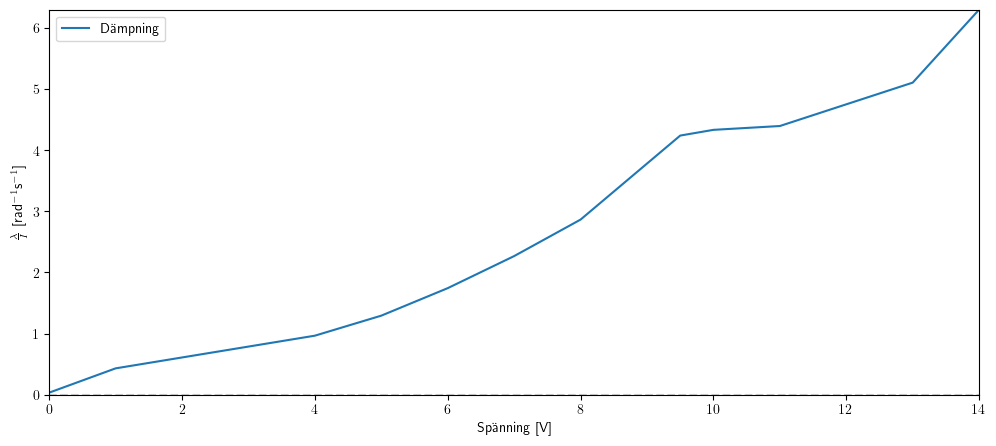
\includegraphics[width=\textwidth]{graf_voltage_damping}
    \caption{Värden på $\frac{\lambda}{I}$ för olika spänning i dämpningsenheten.}
    \label{fig:dämpning_över_spänning}
\end{figure}

\section{Slutsatser}

\end{document}